\documentclass[journal]{IEEEtran}

\usepackage{amsmath,amsfonts}
\usepackage{booktabs}
\usepackage{graphicx}
\usepackage{multirow}
\usepackage{xcolor}
\usepackage{tikz}
\usetikzlibrary{arrows.meta,positioning,fit,calc}

\title{Block-Missing Imputation of Antarctic Automatic Weather Station Records with ERA5 Reanalysis Conditioning}

\author{Anonymous Authors}

\begin{document}
\maketitle

\begin{abstract}
Antarctic automatic weather stations (AWSs) provide essential in situ meteorological observations, but their records are frequently interrupted by sensor icing, power failures, and maintenance gaps that produce contiguous multi-day outages. We study block-wise imputation of 3-hourly Antarctic AWS records using ERA5 reanalysis as an external physical prior. We construct an AntAWS-derived benchmark comprising 32 selected stations with aligned ERA5 time series, realistic block-missing simulation, and held-out station splits. Under matched block-missing training, ERA5 conditioning reduces overall MAE from 0.346 to 0.258, with the relative benefit growing from 13.8\% for 24-hour gaps to 26.4\% for 216-hour gaps and concentrating in temperature, wind speed, and specific-humidity channels. Fair ERA5-augmented evaluations of SAITS and iTransformer show that this gain is attributable to ERA5 access and block-missing curriculum matching rather than to any specific fusion architecture: SAITS+ERA5 achieves 0.245 MAE, while iTransformer+ERA5, gated ECBIT, and concat ECBIT cluster near 0.258. Critically, models trained with point-wise MCAR masks transfer poorly to block tests (MAE 0.407 even with ERA5), demonstrating that failure-mode curriculum matching is a prerequisite for effective reanalysis conditioning.
\end{abstract}

\begin{IEEEkeywords}
Antarctica, automatic weather station, ERA5, imputation, transformers, missing data.
\end{IEEEkeywords}

\section{Introduction}

Continuous near-surface meteorological observations are central to Antarctic climate analysis, model evaluation, and field operations. Automatic weather stations (AWSs) extend coverage beyond staffed stations, but the same remoteness that makes them valuable also makes their records incomplete. The AntAWS compilation aggregates Antarctic AWS observations at 3-hourly, daily, and monthly resolutions and documents the role of AWS networks in resolving remote Antarctic conditions \citep{wang2023antaws}. In the selected 3-hourly stations used in this work, missingness is not well described by independent random points: wind speed and relative humidity contain long contiguous gaps, and several stations exhibit outage blocks lasting days to weeks.

The task is imputation, not forecasting: the model reconstructs missing station observations within a window while leaving available observations unchanged. ERA5 reanalysis provides a physically coherent meteorological background \citep{hersbach2020era5}, but using it naively can be counterproductive: when AWS observations are present, ERA5 often duplicates already available temperature and pressure information; when relative humidity is biased, always-on fusion can inject error. We therefore use ERA5 as a conditional prior that is activated by missingness.

For reproducibility, the study uses ECBIT, the ERA5-conditioned block imputation transformer, as a lightweight dual-stream architecture for sparse Antarctic AWS time series. One stream encodes normalized AWS values, observation masks, and time features; the other encodes aligned ERA5 variables. A conditioning module projects ERA5 tokens into the AWS embedding space, and a missing-variable gate restricts ERA5 influence to channels that contain missing positions. Loss is computed only on artificially hidden positions that were genuinely observed in the raw record, so the benchmark and label support remain fixed while ERA5 access, fusion form, and mask curriculum are varied independently.

The current benchmark contains 32 selected AntAWS stations with at least 10 years of record and sufficient multi-variable completeness. Five geographically diverse stations are reserved for held-out generalization. ERA5 point time series are downloaded and aligned to the exact AntAWS 3-hourly timestamps, producing 41,388 sparse 168-step windows. The experimental matrix covers interpolation, last-observation-carried-forward, ERA5 direct substitution, SAITS \citep{du2023saits}, an iTransformer-style imputation baseline \citep{liu2024itransformer}, ERA5-augmented SAITS/iTransformer controls, and ECBIT ablations.

The contributions are:
\begin{itemize}
  \item an AntAWS-derived benchmark of 32 selected 3-hourly stations with aligned ERA5 point series, sparse observation masks, realistic block-missing simulation, and held-out station splits;
  \item quantitative evidence that ERA5 conditioning reduces block-trained MAE from 0.346 to 0.258, with a relative benefit that grows from 13.8\% at 24 h to 26.4\% at 216 h, concentrated in temperature, wind speed, and specific humidity;
  \item a failure-mode curriculum study showing that MCAR-trained ERA5 models transfer poorly to block tests, reaching 0.407 MAE, whereas block-trained ERA5 models reach 0.258;
  \item fair ERA5-augmented baseline tests showing that augmented SAITS, augmented iTransformer, gated ECBIT, and concat ECBIT are statistically indistinguishable in aggregate MAE, placing the empirical emphasis on failure-mode matching and ERA5 conditioning rather than fusion architecture.
\end{itemize}

\section{Related Work}

\subsection{Polar AWS Records and Reanalysis Products}
Antarctic AWS records are indispensable for evaluating surface meteorology in regions where staffed stations are sparse. AWS networks provide the only sustained in situ observations for many coastal, ice-shelf, and interior locations, but their records are also shaped by the same environmental constraints that make them valuable: winter darkness, icing, snow burial, power interruptions, and infrequent maintenance access. The AntAWS dataset compiles quality-controlled AWS observations across Antarctica and provides 3-hourly meteorological variables including air temperature, pressure, relative humidity, and wind \citep{wang2023antaws}. The IMAU Antarctic AWS archive adds a complementary long-term record with additional surface-energy and surface-height variables at 19 locations from 1995--2022 \citep{vantiggelen2025imau}. Although Greenland is not the target region of this work, the PROMICE and GC-NET AWS archives are important methodological comparators because they document the kind of sensor metadata, quality-control logic, station redesign, and operational data release practices expected for polar station datasets \citep{fausto2021promice,fausto2026promicegcnet}.

Reanalysis products provide spatially complete, physically constrained background fields that are attractive for sparse polar settings. ERA5 provides hourly global atmospheric variables and is widely used as a modern reanalysis baseline \citep{hersbach2020era5}. However, Antarctic validation studies show that reanalysis should not be treated as ground truth. ERA5 near-surface temperature over Antarctica has high monthly correlation with station observations but exhibits regionally structured biases \citep{zhu2021era5antarctica}. In the Antarctic Peninsula--Ellsworth Land region, ERA5 performance depends on parameter and geographic context \citep{tetzner2019era5antarcticpeninsula}. Coastal wind studies likewise show that ERA5 can be the strongest available reanalysis while still missing local variability near complex orography and coastal margins \citep{catonharrison2022antarcticwinds}. These findings support the design choice in ECBIT: ERA5 should be used as a conditional prior during outages, not as a wholesale replacement for AWS observations.

Recent climate-data reconstruction work further motivates combining sparse observations with physically coherent gridded products. \citet{ma2025antarcticsat} train a deep model with reanalysis fields and observation masks to reconstruct Antarctic surface air temperature from sparse in situ records. \citet{li2026era5superresolution} study super-resolution transferability for ERA5, highlighting the broader role of machine learning in refining reanalysis information across regions and variables. ECBIT differs from these gridded reconstruction and downscaling tasks because its target is station-level temporal imputation inside sparse AWS windows, where observed AWS values must be preserved and ERA5 should be activated only for missing variables and timesteps.

\subsection{Time-Series Imputation}
Classical imputation baselines such as linear interpolation and last-observation-carried-forward are strong sanity checks for short gaps but do not model cross-variable structure. Non-parametric methods such as MissForest can exploit cross-sectional feature relations but are not designed around ordered temporal dynamics \citep{stekhoven2012missforest}. Deep imputation methods add temporal modeling and learned latent structure. GRU-D incorporates missingness indicators and time gaps into recurrent modeling \citep{che2018grud}. BRITS learns missing values inside a bidirectional recurrent computation graph \citep{cao2018brits}. SAITS uses self-attention and missingness-aware weighting for multivariate time-series imputation \citep{du2023saits}. GP-VAE and CSDI frame imputation probabilistically through latent-variable or score-based generative modeling \citep{fortuin2020gpvae,tashiro2021csdi}.

Survey and benchmark work makes clear that time-series imputation performance is tightly coupled to missingness assumptions. \citet{fang2020imputationsurvey} review deep imputation architectures and their treatment of temporal structure, while \citet{wang2024imputationsurvey} organize multivariate imputation methods by uncertainty modeling and neural architecture. TSI-Bench standardizes deep imputation evaluation across many algorithms, datasets, and missingness scenarios \citep{du2024tsibench}. Its scale is valuable, but ECBIT addresses a different question. TSI-Bench asks how generic imputation algorithms compare under benchmark missingness protocols; ECBIT asks whether a domain-specific block-missing curriculum and ERA5 conditioning improve Antarctic AWS recovery under realistic contiguous station outages. The protocols are therefore complementary rather than interchangeable.

\subsection{Transformers for Time Series}
ECBIT uses transformer encoders because self-attention provides a flexible mechanism for variable-level interaction and long-window context modeling \citep{vaswani2017attention}. Time-series transformers have evolved away from direct transplantation of language-model tokenization. Informer and Autoformer introduced efficient attention and decomposition ideas for long-sequence forecasting \citep{zhou2021informer,wu2021autoformer}. FEDformer combines decomposition and frequency-domain attention for long-horizon forecasting \citep{zhou2022fedformer}. PatchTST segments time series into patch tokens and uses channel-independent sharing for efficient long-context modeling \citep{nie2023patchtst}. TimesNet maps one-dimensional temporal variation into two-dimensional periodic structures and reports broad performance across forecasting, imputation, classification, and anomaly detection \citep{wu2023timesnet}. iTransformer inverts the standard representation and treats each variate as a token, allowing attention to operate over variables rather than individual timestamps \citep{liu2024itransformer}.

The variate-token choice is natural for AWS imputation because the core physical couplings are cross-variable: temperature, pressure, humidity, and wind are not independent channels. ECBIT adopts the iTransformer-style variate-token view, but it changes the task from forecasting to reconstruction under sparse observation masks. Each token contains a full 168-step trajectory plus mask and time features. This allows the model to learn variable-level relationships without treating every timestamp as a separate attention token.

\subsection{Exogenous Conditioning and Domain-Specific Restoration}
Recent work on auxiliary information in time series cautions against unconstrained fusion. \citet{lee2026constrainedfusion} report that naive multimodal fusion can underperform when auxiliary modalities inject irrelevant information, and propose the Controlled Fusion Adapter (CFA) for time-series forecasting settings. \citet{cao2026ecto} motivate physically grounded selection of meteorological exogenous variables rather than treating all auxiliary channels as uniformly useful. \citet{chen2025exost} identify inconsistent effects across exogenous variables and propose a ``select, then balance'' ExoST framework that dynamically selects and balances exogenous signals.

Meteorological restoration work provides a closer domain analogue. ST-DAN combines a transformer temporal path with a graph-attention path to restore buoy meteorological data using ERA5 and in situ observations \citep{song2026stdan}. ECBIT shares the motivation that physical variables and external reanalysis can help data restoration, but differs in three respects. First, it targets Antarctic AWS outages rather than marine buoy records. Second, it explicitly evaluates block-missing training against MCAR training, showing that the missingness curriculum is itself a major factor. Third, the ablation results show that a lightweight conditioning mechanism is sufficient once ERA5 alignment and block-curriculum matching are correct. The empirical value therefore lies less in a complex fusion block and more in matching the physical failure mode while controlling how external meteorological context enters the model.

\section{Data and methods}

\subsection{Station Selection}
The benchmark is constructed from the 3-hourly AntAWS station archive \citep{wang2023antaws}. The raw archive contains 267 station files after metadata matching and file-level screening. We retain stations only when they provide at least ten years of records, at least 70\% temperature completeness, at least 50\% mean completeness over the core variables, at least 20\% completeness for every core variable, and valid geographic metadata. Applied sequentially, these filters reduce the station pool from 267 to 117 after the record-length threshold, to 38 after the temperature-completeness threshold, to 36 after the core-mean threshold, and finally to 32 after the per-variable completeness threshold. The criteria remove stations that are long but effectively unusable for multivariate imputation, such as stations with nearly absent relative humidity records.

The final benchmark contains 32 stations. Twenty-seven stations are used for the main train/validation/test experiments, and five geographically separated stations are reserved for held-out generalization: Butcher Ridge, Mount Sidley, Nico, Sabrina, and Zhongshan. The held-out set was fixed before training by applying geographic farthest-point sampling to the eligible station set. It provides a station-level transfer test across separated Antarctic locations.

Table~\ref{tab:station-metadata} summarizes the selected station population. Appendix Table~\ref{tab:station-metadata-full} reports the full station-level metadata, temporal coverage, variable completeness, and split assignment.

\begin{table}[t]
  \centering
  \caption{Benchmark station summary. Completeness values are mean observed fractions over retained raw 3-hourly station records; full station metadata are reported in Appendix Table~\ref{tab:station-metadata-full}.}
  \label{tab:station-metadata}
  \begin{tabular}{lrrrrrr}
    \toprule
    Split & Stations & Years & Elev. & T & RH & q \\
    & & & (m) & (\%) & (\%) & (\%) \\
    \midrule
    held-out & 5 & 1989--2021 & 2030 & 78 & 82 & 70 \\
    main & 27 & 1984--2021 & 416 & 79 & 70 & 61 \\
    \bottomrule
  \end{tabular}
\end{table}


\subsection{ERA5 Alignment}
For each selected station, we download an ERA5 single-level point time series \citep{hersbach2020era5} using the CDS time-series API at the station latitude and longitude. The requested ERA5 variables are 2 m temperature, surface pressure, 2 m dewpoint temperature, and 10 m zonal and meridional wind. These variables are converted to the model channels used by AWS: temperature in $^\circ$C, relative humidity in percent, wind speed in m s$^{-1}$, pressure in hPa, and specific humidity in g kg$^{-1}$. Wind speed is computed from the two 10 m wind components. Relative humidity and specific humidity are derived from ERA5 temperature, dewpoint, and pressure using Bolton's saturation-vapor-pressure approximation \citep{bolton1980computation}, matching the AWS-derived humidity preprocessing.

The downloaded CDS point series is used as the ERA5 record for the station coordinates. The hourly ERA5 values are linearly interpolated to the exact AntAWS 3-hourly timestamps. All ERA5 files are checked for finite values and for matching temporal length before preprocessing. ERA5 and AWS channels are normalized with the same variable-wise statistics computed from main-station chronological training segments only. Held-out stations are excluded from those normalization statistics and from all model training.

In the benchmark windows, AWS observations define the target values at observed positions. The aligned ERA5 sequence is stored as an external meteorological background for the same timestamps.

AWS specific humidity is derived during preprocessing from temperature, relative humidity, and pressure using the same saturation-vapor-pressure formula and is stored in g kg$^{-1}$. Its observation mask is the intersection of the source-variable masks: if any required source value is missing or non-finite, the derived $q$ value is marked missing. Artificial masks are sampled after this derivation on the five-channel benchmark representation. The ERA5 $q$ channel is aligned and normalized with the same train-window statistics as the AWS-derived $q$ target.

\subsection{Sparse Window Generation}
Strictly complete windows are rare in Antarctic AWS records. Requiring every variable to be observed for a full 168-step window would leave few windows and bias the benchmark toward unusually clean periods, so windows are generated with explicit observation masks.

Each window contains $T=168$ 3-hourly steps, corresponding to three weeks. The preprocessing stride is 42 steps, or one quarter of the window length. Windows are retained when at least 25\% of all variable-time positions are observed, at least three variables have at least 12 observed steps inside the window, and the station belongs to the selected main or held-out split. Within each station, retained windows are ordered chronologically and assigned to 70\% train, 10\% validation, and 20\% test segments. The final preprocessing output contains 41,388 windows with normalized AWS values, binary observation masks, aligned ERA5 sequences, timestamp encodings, start indices, start timestamps, and split identifiers. Artificial masks are sampled from observed positions in this window representation.

Table~\ref{tab:split-overlap-audit} reports the chronological split gaps and sliding-window overlap. For every station, the validation segment lies between the training and test segments; the minimum train--test gap is 2268 steps, which is much longer than the 168-step input window. Validation and test windows can overlap because windows are generated with a 42-step stride. We also define a deterministic non-overlapping test subset by retaining test windows with start times separated by at least 168 steps. This subset contains 2102 windows, or 25.3\% of the original test windows.

\begin{table}[t]
  \centering
  \caption{Chronological split-overlap audit. Gaps are measured between the end of the earlier split window and the start of the later split window within each station. Negative values indicate context overlap. The non-overlap subset greedily retains test windows separated by at least one 168-step window length.}
  \label{tab:split-overlap-audit}
  \footnotesize
  \setlength{\tabcolsep}{3pt}
  \begin{tabular}{@{}p{0.36\linewidth}p{0.39\linewidth}p{0.18\linewidth}@{}}
    \toprule
    Quantity & Value & Stations \\
    \midrule
    Test windows & 8307 & 32 \\
    Non-overlap subset & 2102 (25.3\%) & 32 \\
    Test stride & median 42 steps & 32 \\
    Train--test gap & min 2268; median 4767 steps & 0 overlap \\
    Val--test gap & min -126; median -126 steps & 32 overlap \\
    \bottomrule
  \end{tabular}
\end{table}


\subsection{Observed Missingness}
The selected records contain many contiguous gaps. Wind speed and relative humidity carry the largest missing burden, with 90th-percentile gap lengths exceeding two days (Fig.~\ref{fig:missing-patterns}). This pattern motivates block-wise artificial masks for the main experiments. The observed mask records which AWS values are available in each sparse window.

\begin{figure}[t]
  \centering
  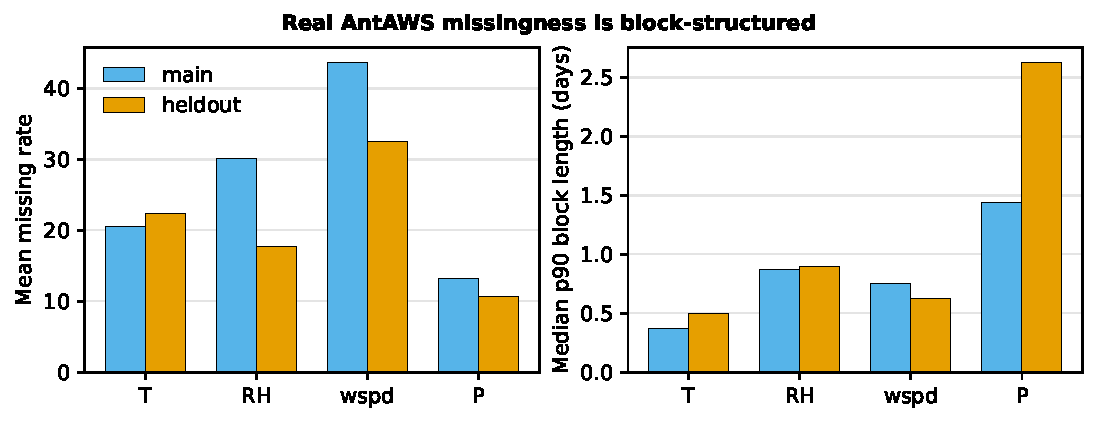
\includegraphics[width=\columnwidth]{figures/fig_missing_patterns.pdf}
  \caption{Observed missingness in selected AntAWS stations. Wind speed and relative humidity show the largest missing burden, and high-percentile gaps last multiple days, motivating block-wise rather than point-wise imputation.}
  \label{fig:missing-patterns}
\end{figure}

\section{Methodology}

\subsection{Problem Formulation}
Let $X \in \mathbb{R}^{T \times C}$ be a normalized AWS window with $T=168$ 3-hourly steps and $C=5$ variables: temperature, relative humidity, wind speed, pressure, and specific humidity. Let $O \in \{0,1\}^{T \times C}$ denote the real observation mask, where $O_{t,c}=1$ means the station value is observed. ERA5 provides an aligned dense sequence $E \in \mathbb{R}^{T \times C}$. During training and evaluation, we sample an artificial missing mask $A$ only from positions where $O=1$. The model input mask is
\begin{equation}
M = (1 - O) \lor A,
\end{equation}
and the supervised loss is computed only on $A$:
\begin{equation}
\mathcal{L} = \frac{\sum_{t,c} A_{t,c}(\hat{X}_{t,c}-X_{t,c})^2}{\sum_{t,c} A_{t,c}}.
\end{equation}
This avoids treating real unobserved values as ground truth.

\subsection{Block Missing Simulation}
Real AntAWS missingness is block-structured. We therefore sample contiguous outage blocks with three regimes: short gaps of 6--24 steps, medium gaps of 24--72 steps, and long gaps of 72--240 steps. Missing rates are set to 20\%, 40\%, and 60\%. A point-wise MCAR mask is used only for the no-blockmask ablation.

\subsection{ECBIT Architecture}
ECBIT uses two variate-token encoders. For each variable $c$, the observation token is formed from its full time series, the observation mask, and shared time encodings. ERA5 tokens are formed from the aligned ERA5 variable and the same time encodings. Transformer encoders produce $Z^{aws}, Z^{era5} \in \mathbb{R}^{C \times d}$.

Conditional fusion applies cross-attention with AWS as query and ERA5 as key/value:
\begin{equation}
H = \mathrm{MHA}(Q=Z^{aws}, K=Z^{era5}, V=Z^{era5}).
\end{equation}
A variable-level gate $g_c=\mathbb{1}[\sum_t M_{t,c}>0]$ controls whether ERA5 can alter the AWS representation:
\begin{equation}
Z_c = \mathrm{LayerNorm}(Z^{aws}_c + g_c H_c).
\end{equation}
The reconstruction head maps each variable token back to a length-$T$ sequence. If a variable has no missing positions, its output is independent of ERA5 after fusion.

\section{Experimental Protocol}

\subsection{Evaluation Setting}
All reported neural results are evaluated on held-out test windows using the checkpoint selected by validation performance. Metrics are computed only on artificially hidden positions that were observed in the original AWS record. We report normalized mean absolute error (MAE) and root mean squared error (RMSE), averaged over variables unless otherwise specified.

The main block-missing experiments use three outage regimes: short, medium, and long blocks. Missing rates are 20\%, 40\%, and 60\%, with three random seeds for each configuration. The held-out station experiment evaluates transfer to five stations excluded from model training at 40\% block missingness.

\subsection{Baselines}
We compare against four core baselines. Linear interpolation and last-observation-carried-forward test whether local temporal continuity is sufficient. ERA5 direct substitution fills missing positions with bias-corrected ERA5 values while preserving observed AWS values, testing the strength of reanalysis alone. The iTransformer imputation baseline tests a neural variate-token model without ERA5 conditioning.

We also implemented wrappers for BRITS and SAITS, but the current completed result matrix focuses on the baselines above and the ECBIT ablations. This avoids mixing incomplete third-party baseline runs into the main claims. BRITS and SAITS remain relevant methodological references because they represent recurrent and self-attention imputation families, respectively.

\subsection{Ablations and Follow-up Analyses}
The primary ECBIT ablation compares gated ERA5 injection, concat/no-cross fusion, and no-ERA5 training under matched block-missing conditions. A no-blockmask variant trains with MCAR masks and is reported separately because its training distribution differs from the block-failure regime.

To explain the ERA5 signal, we run three follow-up analyses. First, block-length sensitivity varies the maximum outage horizon from 24 to 216 hours while comparing ERA5-conditioned and no-ERA5 models. Second, ERA5 variable masking replaces one ERA5 channel at inference time with its training-set mean to measure channel importance. Third, ERA5 temporal downsampling evaluates whether the model depends on high-frequency ERA5 structure or only on a coarser background state.

\section{Experiments}

\subsection{Data}
We scan 267 AntAWS 3-hourly station files and retain stations with record length of at least 10 years, temperature completeness of at least 70\%, mean core-variable completeness of at least 50\%, and minimum core-variable completeness of at least 20\%. This yields 27 main stations and five held-out stations: Butcher Ridge, Mount Sidley, Nico, Sabrina, and Zhongshan. ERA5 point time series are aligned to the exact station timestamps and normalized with statistics fitted on main-station train windows.

\begin{figure}[t]
  \centering
  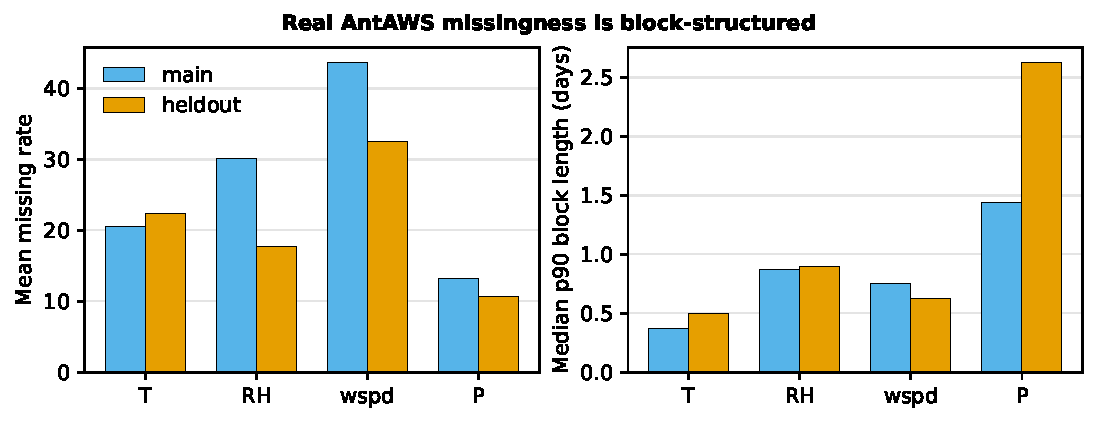
\includegraphics[width=\columnwidth]{figures/fig_missing_patterns.pdf}
  \caption{Observed missingness in selected AntAWS stations. Wind speed and relative humidity show the largest missing burden, and high-percentile gaps last multiple days, motivating block-wise rather than point-wise imputation.}
  \label{fig:missing-patterns}
\end{figure}

\subsection{Baselines and Ablations}
Round 1 compares six baselines: linear interpolation, last-observation-carried-forward, ERA5 direct substitution after train-set bias correction, BRITS, SAITS, and an iTransformer imputation baseline. Round 2 evaluates ECBIT variants: full conditional cross-attention, no cross-attention, no ERA5, and no block-mask training. Round 3 evaluates held-out station generalization for ECBIT full at a 40\% missing rate.

\subsection{Implementation Status}
The data pipeline, model implementations, training/evaluation entrypoints, and 315 YAML experiment configurations have been implemented. Remote GPU execution is pending SSH credential availability. Result tables and statistical comparisons will be added after the remote experiment batches complete.

\section{Discussion}

\subsection{What the ERA5 Signal Represents}
The results support a specific interpretation of ERA5 conditioning. ERA5 is not merely another correlated input channel that improves every setting equally. Its value grows as station outages become longer, precisely when local interpolation and station-history cues weaken. This is consistent with ERA5 acting as a physically coherent background state during multi-day sensor failures.

The variable-masking analysis further shows that the ERA5 contribution is not uniform across variables. Temperature, wind speed, and specific humidity produce the largest MAE increases when removed. Relative humidity is least important among the tested channels, which is consistent with the concern that ERA5 humidity can be biased in polar settings. This supports the decision to condition on ERA5 through missing-variable gates rather than replacing station observations wholesale.

\subsection{Why Complex Fusion Did Not Dominate}
The cross-attention and gated-injection experiments show that the specific fusion mechanism is not the dominant source of improvement. Gated injection and concat/no-cross fusion are statistically tied, while removing ERA5 causes a large degradation. This suggests that once aligned ERA5 information and block-missing training are available, a lightweight conditioning mechanism is sufficient for the present benchmark.

This finding changes the interpretation of the method. The contribution is not that attention-style fusion is intrinsically superior; instead, the contribution is identifying and validating the conditions under which external reanalysis becomes useful for Antarctic AWS imputation. Reporting the negative fusion result is important because it prevents over-claiming architectural novelty and makes the empirical conclusion more robust.

\subsection{Curriculum and Failure-Mode Matching}
The MCAR-on-block evaluation shows that ERA5 conditioning alone is insufficient. A model trained with MCAR masks performs poorly when evaluated on block-missing tests, even though it has access to ERA5. This indicates an interaction between the external physical prior and the missingness curriculum: the model must learn to use ERA5 under contiguous outage conditions, not only under randomly scattered missing points.

For practical Antarctic AWS recovery, this matters more than performance on generic random-missing benchmarks. Station failures often remove contiguous spans of one or more variables, so evaluation and training should match that failure mode.

The completed factorial matrix makes this conclusion quantitative. Block-missing curriculum has a larger average main effect than ERA5 conditioning (0.166 versus 0.105 MAE), while their effect-coded interaction is positive but small (0.017 MAE). This is methodologically useful beyond the present dataset: exogenous variables can be valuable, but their value depends on whether the training mask distribution teaches the model how to use them under the target failure mode.

\subsection{Practical Deployment Considerations}
The temporal-resolution analysis suggests that ECBIT does not require fragile hour-level ERA5 structure. Downsampling ERA5 to 6-hour resolution changes MAE by less than 0.001, while daily inputs are clearly too coarse. This supports practical deployments where only lower-frequency reanalysis products or delayed operational reanalysis streams are available, provided that sub-daily temporal structure is preserved.

The variable-importance results also suggest a prioritization rule for partial ERA5 availability. Temperature, wind speed, and specific humidity are the most valuable channels and account for about 84\% of the total single-channel masking degradation; pressure and relative humidity contribute less in the current benchmark. If a deployment pipeline must reduce ERA5 variables, the top three channels should be preserved first.

The held-out station results further suggest that deployment should include station-level validation. Mean MAE ranges from 0.173 to 0.350 across the five held-out stations, so high-elevation, coastal, or locally complex stations should be checked before operational use rather than assumed to follow the aggregate benchmark average.

\subsection{Station Heterogeneity}
Held-out station results vary by roughly a factor of two, from Nico to Mount Sidley. This heterogeneity likely reflects a combination of local geography, elevation, coastal versus interior climate regimes, and station-specific ERA5 representativeness. Mount Sidley has the largest held-out MAE. In the selected metadata it is also the highest held-out station, at 2123 m, and lies in West Antarctic complex terrain where coarse reanalysis orography and boundary-layer structure can be mismatched to the local AWS footprint. Zhongshan has the second-largest MAE despite its low elevation, plausibly because its coastal setting is affected by sea-ice, ocean, and local wind interactions that are not fully resolved by point-sampled ERA5. Future work should therefore consider station-adaptive conditioning, metadata-aware calibration, or few-shot adaptation for stations with large ERA5 bias.

\subsection{Limitations}
The benchmark uses artificial masks on originally observed positions, which provides controlled ground truth but does not directly evaluate recovery inside historical gaps where no AWS observation exists. ERA5 is aligned at station points and shares the selected variable set; other reanalysis products, spatial interpolation strategies, or station metadata may change the optimal conditioning strategy. Finally, the completed result matrix prioritizes a controlled 2$\times$2 curriculum-by-ERA5 factorial design over a broad third-party imputation suite. BRITS and SAITS wrappers are implemented, but complete block-curriculum retraining and evaluation for those methods is left for future benchmarking; the current study isolates why ERA5 and block-missing curriculum matter before expanding the model zoo.

\section{Conclusion}

We introduced ECBIT, an ERA5-conditioned framework for sparse Antarctic AWS block imputation. The empirical results show that ERA5 provides the dominant improvement signal: removing ERA5 substantially degrades block-imputation accuracy, while gated and concat fusion perform similarly. Follow-up analyses sharpen this conclusion: ERA5 gains grow with outage length, concentrate in physically meaningful temperature, wind, and humidity channels, and require block-missing curriculum to transfer to block failures. This indicates that the primary value lies in matching the real failure mode and conditioning on reanalysis background state, rather than in a specific attention-style fusion module. Held-out station results further show that Antarctic station generalization is heterogeneous and should be reported explicitly rather than collapsed into a single average.


\appendices
\section{Full Station Metadata}
\begin{table*}[p]
  \centering
  \tiny
  \caption{Selected station metadata for the AntAWS-derived benchmark. Completeness columns report the fraction of observed 3-hourly values in the retained raw station record before sparse-window construction.}
  \label{tab:station-metadata-full}
  \begin{tabular}{lrrrrrrrrrrl}
    \toprule
    Station & Lat. & Lon. & Elev. & Start & End & T & RH & Wind & P & q & Split \\
    & (deg) & (deg) & (m) & & & (\%) & (\%) & (\%) & (\%) & (\%) & \\
    \midrule
    Butcher Ridge & -79.15 & 155.89 & 2030 & 2008 & 2021 & 75 & 93 & 53 & 93 & 75 & held-out \\
    Mount Sidley & -77.13 & -125.97 & 2123 & 2010 & 2020 & 78 & 89 & 69 & 93 & 75 & held-out \\
    Nico & -89.00 & 90.02 & 2979 & 1993 & 2021 & 78 & 86 & 79 & 86 & 78 & held-out \\
    Sabrina & -84.24 & -170.26 & 87 & 2009 & 2021 & 83 & 84 & 78 & 95 & 66 & held-out \\
    Zhongshan & -69.37 & 76.38 & 18 & 1989 & 2020 & 74 & 59 & 58 & 80 & 54 & held-out \\
    Alessandra & -73.59 & 166.62 & 160 & 1987 & 2021 & 83 & 89 & 49 & 92 & 81 & main \\
    Arelis & -76.72 & 162.97 & 150 & 1990 & 2021 & 93 & 52 & 26 & 97 & 50 & main \\
    Bear Peninsula & -74.55 & -111.87 & 416 & 2011 & 2021 & 73 & 68 & 30 & 77 & 64 & main \\
    Cape Bird & -77.22 & 166.44 & 38 & 1999 & 2021 & 86 & 49 & 68 & 89 & 44 & main \\
    Clean Air & -90.00 & 0.00 & 2835 & 1986 & 2005 & 79 & 46 & 86 & 76 & 30 & main \\
    Eneide & -74.70 & 164.09 & 91 & 1987 & 2021 & 89 & 89 & 26 & 95 & 86 & main \\
    Erin & -84.90 & -128.87 & 988 & 1994 & 2021 & 72 & 41 & 57 & 42 & 39 & main \\
    Gill & -79.82 & -178.54 & 53 & 1985 & 2021 & 72 & 21 & 62 & 88 & 16 & main \\
    Harry & -83.01 & -121.41 & 956 & 1994 & 2021 & 74 & 49 & 64 & 76 & 43 & main \\
    Henry & -89.00 & -0.41 & 2781 & 1993 & 2021 & 75 & 66 & 61 & 82 & 62 & main \\
    Howard Nunatak & -77.53 & -86.77 & 1502 & 2010 & 2021 & 88 & 99 & 73 & 99 & 88 & main \\
    Laurie II & -77.43 & 170.74 & 34 & 2000 & 2021 & 72 & 91 & 73 & 92 & 72 & main \\
    Lola & -74.14 & 163.43 & 1621 & 1990 & 2021 & 89 & 41 & 26 & 94 & 39 & main \\
    Lower Thwaites Glacier & -76.44 & -107.77 & 999 & 2009 & 2021 & 71 & 80 & 59 & 80 & 71 & main \\
    Manuela & -74.95 & 163.69 & 78 & 1984 & 2021 & 83 & 34 & 31 & 88 & 32 & main \\
    Marble Point II & -77.44 & 163.76 & 111 & 2011 & 2021 & 84 & 92 & 81 & 94 & 83 & main \\
    Margaret & -79.98 & -165.10 & 67 & 2008 & 2021 & 77 & 100 & 79 & 100 & 77 & main \\
    Minna Bluff & -78.55 & 166.69 & 895 & 1991 & 2020 & 72 & 49 & 39 & 82 & 44 & main \\
    Silvia & -73.05 & 169.60 & 568 & 1990 & 2021 & 80 & 68 & 22 & 83 & 65 & main \\
    Sofia & -74.82 & 163.23 & 40 & 1987 & 2002 & 80 & 91 & 25 & 83 & 73 & main \\
    Theresa & -84.60 & -115.85 & 1454 & 1994 & 2021 & 83 & 88 & 81 & 88 & 83 & main \\
    Thurston Island & -72.53 & -97.55 & 225 & 2011 & 2021 & 91 & 85 & 27 & 99 & 77 & main \\
    Up Thwaites Glacier & -77.58 & -109.03 & 1314 & 2010 & 2020 & 72 & 87 & 52 & 87 & 72 & main \\
    Vito & -78.41 & 177.83 & 50 & 2004 & 2021 & 74 & 90 & 78 & 86 & 65 & main \\
    aws05 & -73.10 & -13.17 & 360 & 1998 & 2014 & 79 & 87 & 85 & 93 & 73 & main \\
    aws06 & -74.47 & -11.52 & 1160 & 1998 & 2009 & 76 & 86 & 87 & 92 & 71 & main \\
    aws11  & -71.17 & -6.80 & 690 & 2007 & 2019 & 81 & 50 & 77 & 89 & 44 & main \\
    \bottomrule
  \end{tabular}
\end{table*}



\bibliographystyle{IEEEtran}
\bibliography{references}

\end{document}
